\chapter{Basi di elaborazione del segnale}
\pagenumbering{arabic}
\label{math_bkg}
In questo capitolo introdurremo alcuni concetti basilari sull'elaborazione dei
segnali necessari alla comprensione del funzionamento di uno
spettrometro e del suo campo di applicazione. Sapere cosa sia un segnale, come
si estraggono ed elaborano le informazioni in esso contenuto o quali siano i
concetti matematici utilizzati \`e fondamentale per capire il lavoro svolto.\\
Questo materiale introduttivo \`e sufficiente per avere una panoramica sui
concetti teorici utilizzati.

\section{Segnali}
Il nostro corpo \`e in grado di percepire, attraverso i sensi, alcune delle
variazioni nelle propriet\`a fisiche del mondo che ci circonda. Queste variazioni che percepiamo vengono
elaborate dal nostro cervello che riesce a ricavarne informazioni utili: In questo modo
siamo in grado di percepire se fa caldo o freddo, se c'\`e luce, se un oggetto
\`e di un colore piuttosto che un altro, ecc. Va notato che in questi segnali
c'\`e una componente fisica (la temperatura) e l'informazione veicolata
(freddo/caldo). \cite{bertoni}
\begin{definitions} \label{def:signal}
Si dice segnale una qualunque quantit\`a che varia nel tempo o nello spazio.
\end{definitions}
Secondo la precedente definizione, quindi, \`e possibile che un segnale non
contenga informazioni utili: in questo caso ci si riferisce al segnale come
\emph{rumore}. Il rumore \`e anche una componente di interferenza o errore su di
un segnale che si cerca di interpretare.

Un segnale viene quindi rappresentato da una funzione $g = f(c)$, ove:
\begin{itemize}
    \item $g$ \`e una variabile dipendente su di una grandezza fisica in
    relazione al tempo o spazio.
    \item $c$ \`e una varaibile indipendente che rappresenta lo spazio o il
    tempo.
    \item $f$ \`e una funzione che associa ad un valore temporale o spaziale $c$
    la corrispondente quantit\`a $g$.
\end{itemize}

Per semplicit\`a di esposizione, d'ora in avanti si far\`a riferimento
unicamente a segnali in relazione al tempo.

\subsection{Segnali periodici}
Una importante classe di segnali sono i segnali periodici. Un segnale \`e
periodico se si ripete in un certo periodo di tempo: definendo $T$ il periodo con
cui si ripete il segnale e con $t$ un qualunque momento nel tempo, per ogni $k$,
vale $f(t) = f(t + kT)$. Un segnale periodico $f(t)$ \`e quindi univocamente
individuato nell'intervallo $-\frac{T}{2} \le t \le \frac{T}{2}$.

Si definisce  \emph{frequenza} di un segnale periodico $f(t)$ il numero di
ripetizioni del periodo $T$ nell'unit\`a di tempo. Risulta quindi:
\[
\nu = \frac{1}{T}
\]
L'unit\`a di misura della frequenza \`e l'Hertz ed indica il numero di cicli
(ripetizioni) al secondo.

\subsection{Frequenza radio}
I segnali elettromagnetici vengono classificati a seconda della loro frequenza
in diverse categorie:
\begin{itemize} 
	\item Frequenze minori di 3 GHz vengono denominate \emph{frequenze radio}.
	\item Frequenze comprese tra 3 GHz e 300 GHz sono denominate
		\emph{microonde}.
	\item Frequenze comprese tra 300 GHz e 400 000 GHz (400 THz) sono denominate
		\emph{infrarossi}.
	\item Frequenze comprese tra 400 THz e 750 THz sono parte dello
		\emph{spettro visibile}.
	\item Frequenze comprese tra 750 THz e 30 000 THz (30 PHz) sono denominate
		\emph{raggi ultravioletti}.
	\item Frequenze comprese tra 30 Phz e 30 000 PHz (30 EHz) sono denominate
		\emph{Raggi X}.
	\item Frequenze superiori ai 30 EHz sono denominate \emph{Raggi Gamma}.
\end{itemize}
Va notato che questi limiti sono solo convenzionali e non hanno una definizione
standard.

\subsubsection{Studio dei corpi celesti}
\begin{figure}[htb]
	\begin{center}
		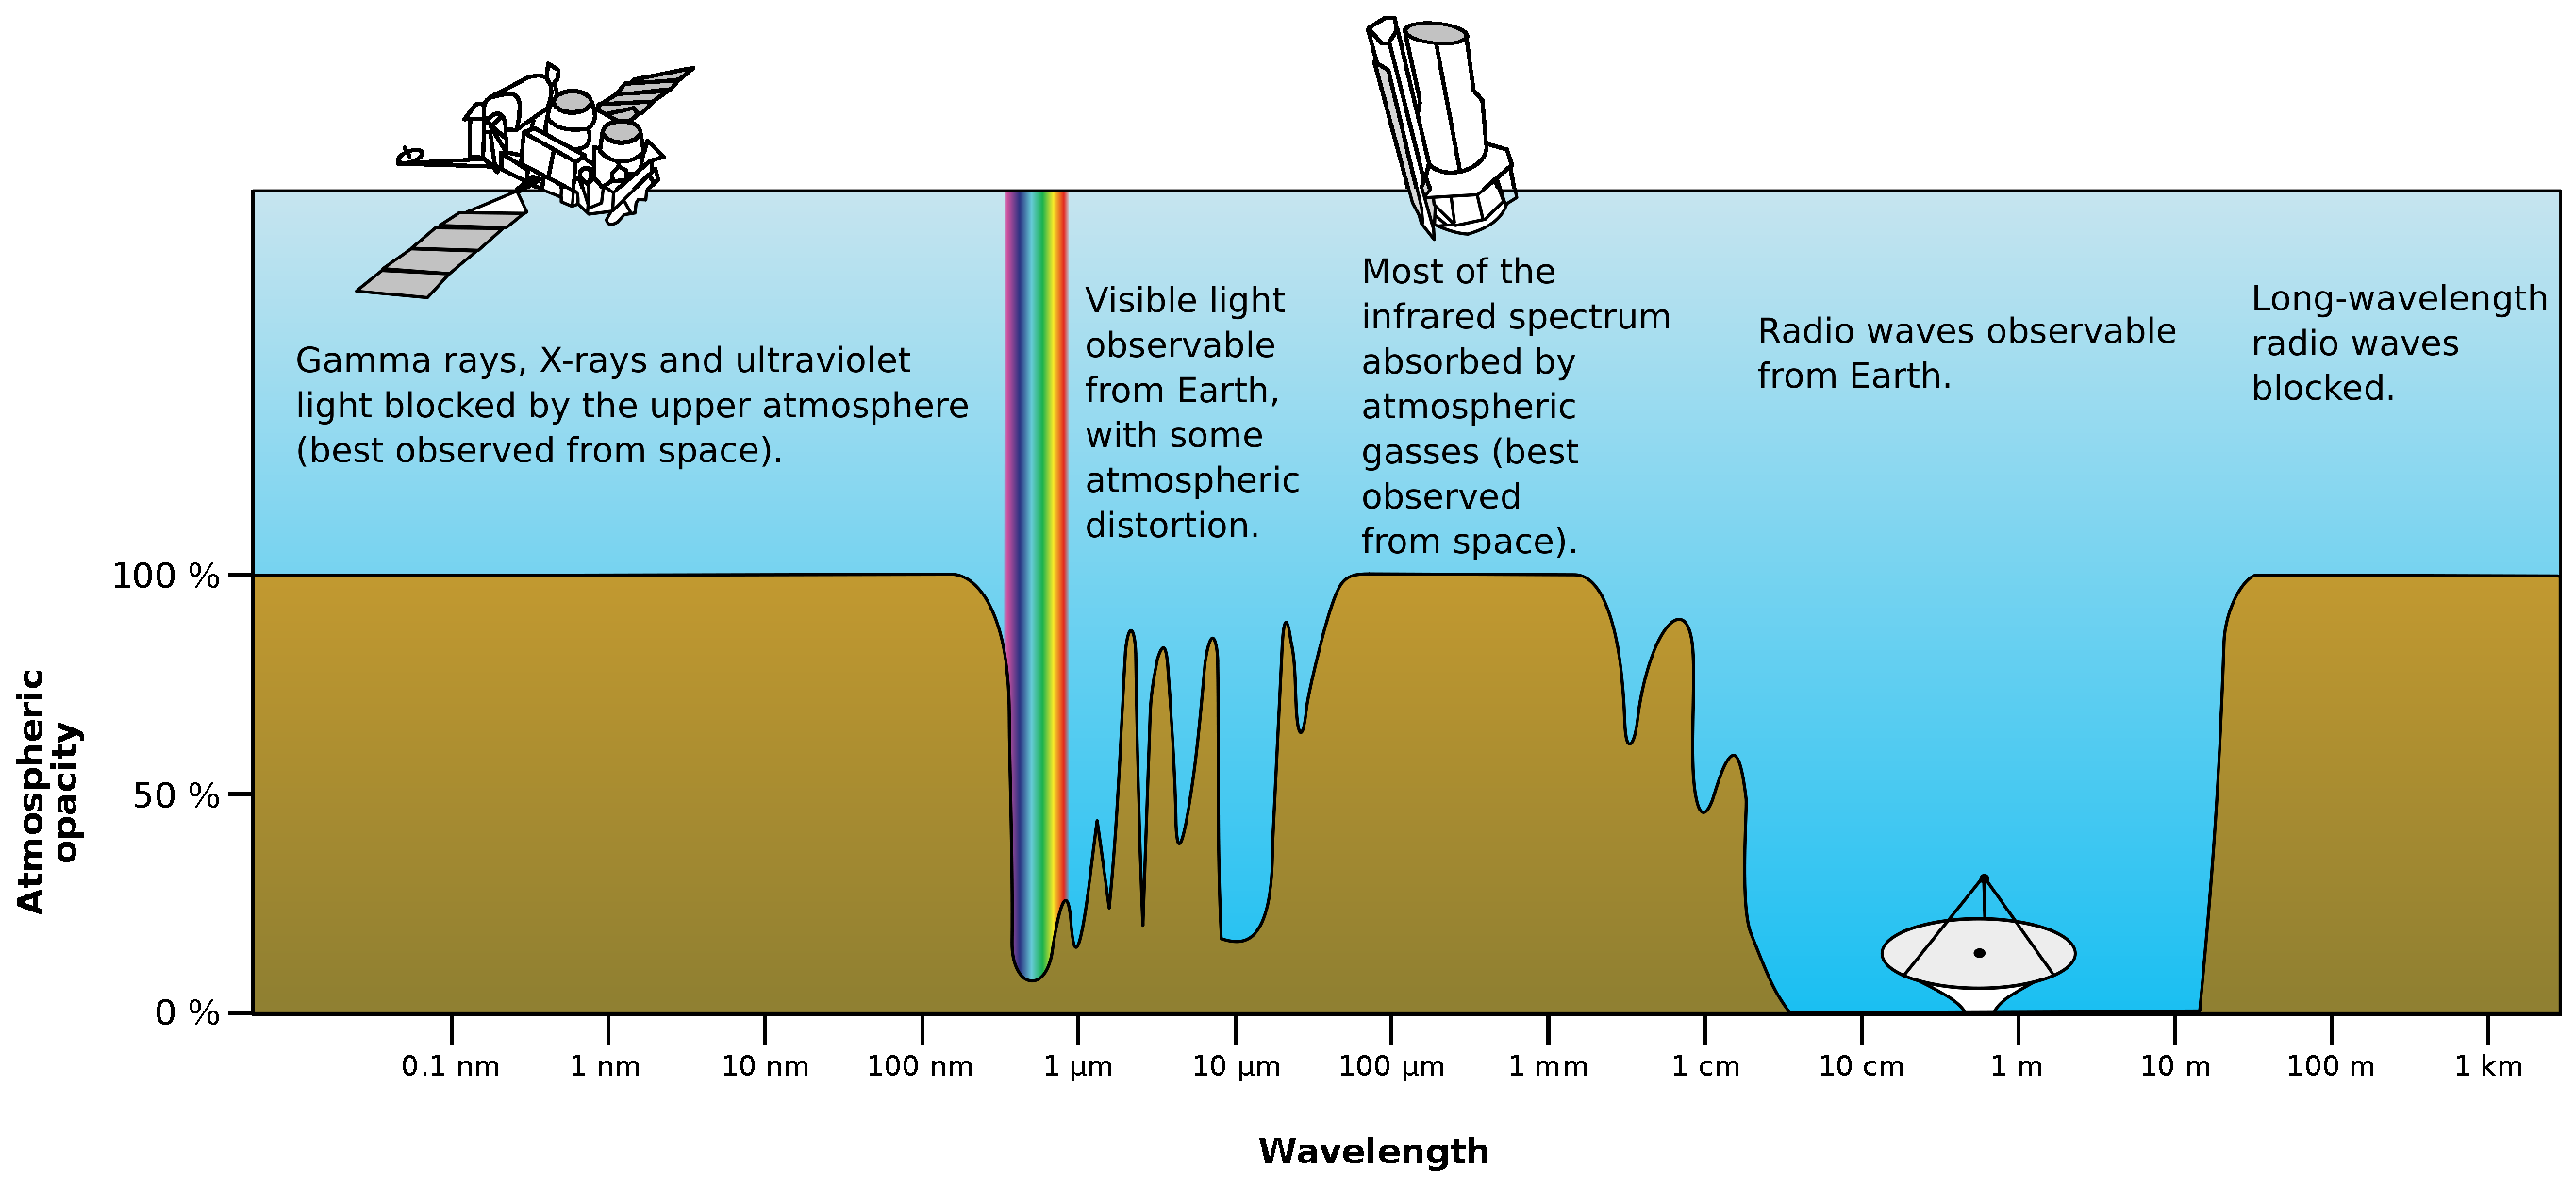
\includegraphics[width=1\linewidth]{Atmospheric_electromagnetic_opacity}
	\end{center}
	\caption{Permeazione dei segnali elettromagnetici nell'atmosfera}
	\label{fig:atm_em_op}
\end{figure}
I segnali elettromagnetici sono fondamentali per lo studio dei corpi celesti.
Tuttavia va considerata la permeabilit\`a dell'atmosfera terrestre rispetto ai
segnali che ci arrivano dallo spazio, come illustrato in Figura
\ref{fig:atm_em_op}\footnote{Fonte:
\url{http://coolcosmos.ipac.caltech.edu/cosmic_classroom/cosmic_reference/irwindows.html}}:
come si pu\`o notare, lo studio dei corpi celesti da terra \`e possibile solo
nello spettro visibile (telescopi, con qualche distorsione) oppure nello spettro
delle frequenze radio (radiotelescopi). Per altre lunghezze d'onda, \`e
necessario studiare questi segnali direttamente dallo spazio con l'ausilio di
satelliti. I moderni radiotelescopi lavorano tra i 70 Mhz ed i 43 Ghz, a seconda
del radiotelescopio, quindi anche le microonde rivestono una qualche importanza
nello studio dei corpi celesti. Questi tipi di segnale sono oggetto di
elaborazione del software sviluppato.

\section{ADC: Analog--to--Digital Conversion}
Per interpretare i segnali del mondo che ci circonda, possiamo sfruttare la
velocit\`a di calcolo di un elboratore; tuttavia per poterlo usare, bisogna
essere in grado di rappresentare le informazioni che riceviamo in modo che
l'elaboratore sia in grado di capirle. Per questo motivo dobbiamo trovare un
modo di trasformare un segnale \emph{analogico} in un segnale \emph{digitale}.

\subsection{Segnali analogici, segnali digitali}
Come abbiamo visto nella definzione \ref{def:signal}, i segnali hanno due
componenti: il tempo e il valore assunto dalla grandezza fisica che osserviamo.
Queste due componenti possono assumere un qualunque valore reale, cio\`e il
segnale ha \emph{tempo continuo} e \emph{valori continui}. Tuttavia, in questo
modo il segnale non pu\`o essere rappresentato da un elaboratore, in quanto un
elaboratore pu\`o contenere solamente quantit\`a finite, mentre le componenti
del segnale sono quantit\`a infinite. Per questo motivo bisogna cercare di far
rientrare il segnale in un range di valori finiti e renderlo cos\`i
rappresentabile da un calcolatore.

Per rendere finita la misurazione del tempo, si possono salvare i valori
rilevati ad un intervallo prefissato, ad esempio una volta ogni secondo.
Misurando un segnale per 10 secondi si otterranno cos\`i 10 valori associati ad
ogni secondo. Un segnale di questo tipo ha \emph{tempo discreto}, ma valori
ancora \emph{continui}. Un dispositivo che raccoglie valori con una determinata
frequenza si chiama \emph{campionatore}.

Per rendere i valori finiti, si pu\`o scegliere di utilizzare un certo insieme
di grandezze, ad esempio $1$ e $-1$, e per ogni valore rilevato, associare la
grandezza pi\`u vicina. Quindi se rileviamo i valori $4$, $10$, $-5$ e $-13$,
salviamo il segnale con i valori $1$, $1$, $-1$, $-1$. Cos\`i facendo, il
segnale assume \emph{valori finiti} che sono rappresentabili in un elaboratore,
nell'esempio fatto con l'uso di 1 bit. Un dispositivo che associa ai valori
rilevati il pi\`u vicino valore rappresentabile dall'elaboratore si chiama
\emph{quantizzatore}.

Un segnale che ha tempo \emph{continuo} e valori \emph{continui} si chiama
\emph{segnale analogico}, mentre un segnale con tempo \emph{discreto} e valori
\emph{finiti} si chiama \emph{segnale digitale}.

Come \`e facile intuire, la conversione da analogico a digitale pu\`o introdurre
degli \emph{errori}, cio\`e del \emph{rumore}, in quanto la versione digitale di
un segnale analogico \`e una approssimazione. Fortunatamente \`e possibile
valutare questo margine di errore e ridurlo a seconda delle necessit\`a sia
aumentando il numero di bit usati per rappresentare i valori nel tempo, sia
aumentando il numero di rilevazioni effettuate nello spazio temporale di
osservazione.

\subsection{Teorema del Campionamento}
Quando si effettua il campionamento di un segnale $f(t)$, si sceglie un periodo
$\tau$ e si fanno $n$ misurazioni nel tempo, ottenendo quindi un segnale di
tipo $f(n\tau)$. Come possiamo assicurarci che da $f(n\tau)$ sia possibile
ricostruire il segnale originale $f(t)$?
Il teorema del campionamento fornisce una risposta definendo un limite basato
sulla frequenza massima del segnale:
\begin{theorem} \label{the:nyquist}
	Un segnale $f(t)$ con frequenza massima $\nu_m$ pu\`o essere ricostruito dal
	segnale campionato $s(n\tau)$ con frequenza $\nu_s = \frac{1}{\tau}$ se
	$\nu_s > 2\nu_m$
\end{theorem}
Cio\`e la frequenza di campionamento deve essere doppia rispetto alla frequenza
massima presente nel segnale.\footnote{Per una dimostrazione del teorema del
campionamento, fare riferimento a \cite{MDFT07}} Nel caso in cui un segnale venga campionato con
frequenza di campionamento $\nu_s < 2\nu_m$, si verifica un fenomeno di
\emph{aliasing}, cio\`e le componenti a frequenza maggiore di $\frac{\nu_s}{2}$
verranno ricostruite come se avessero un'altra frequenza compresa tra $0$ e
$\frac{\nu_s}{2}$; a questo modo l'intero segnale verrebbe compromesso e sarebbe
impossibile recuperare il segnale originario. Per evitare che ci\`o accada si
applica un filtro al segnale che deve essere campionato per eliminare tutte le
frequenze maggiori di $\frac{\nu_s}{2}$, evitando che frequenze non di nostro
interesse possano interferire con le frequenze che andremo ad elaborare.

\section{La Trasformata Discreta di Fourier}
\subsection{Introduzione alla Trasformata di Fourier}
Jean Baptiste Joseph Fourier, vissuto a cavallo tra il XVIII e XIX secolo, era
un matematico francese che, presentando i suoi  studi sulla propagazione del
calore, affermava che qualunque segnale periodico continuo potesse essere
rappresentato come somme pesate di sinusoidi. Questa teoria fu molto osteggiata
da Joseph Louis Lagrange, il quale sosteneva che per segnali contenenti angoli,
come ad esempio le onde quadre, ci\`o non fosse possibile e per questo il
lavoro di Fourier non fu pubblicato per 15 anni, fino alla morte dello stesso
Lagrange.\footnote{cfr. \cite{TSEGDSP97}, capitolo 8} In realt\`a l'approccio di
Fourier non era sbagliato, ma anche l'obiezione di Lagrange \`e valida: se da un
lato \`e vero che un segnale con angoli non potesse essere rappresentato come
somme di sinusoidi, si riesce ad ottenere una approsimazione cos\`i accurata del
segnale da avere una differenza energetica pari a zero.  Questo fenomeno \`e
conosciuto come \emph{Fenomeno di Gibbs}\footnote{cfr.  \cite{TSEGDSP97},
capitolo 11}

\subsection{Tipi di Trasformate di Fourier}
Esistono quattro tipi di segnali possibili, ognuno con la sua trasformata di
Fourier. Un segnale pu\`o essere periodico o aperiodico, continuo o discreto. Ne
conseguono i quattro tipi di trasformate:
\begin{itemize}
	\item \textbf{Aperiodico - Continuo}: Il segnale non \`e periodico ed
		assume infiniti valori. Per analizzarlo si utilizza la \emph{Trasformata
		di Fourier}.
	\item \textbf{Periodico - Continuo}: Il segnale assume infiniti valori che
		si ripetono con un certo periodo. In questo caso si usa la \emph{Serie
		di Fourier}.
	\item \textbf{Aperiodico - Discreto}: Il segnale non ha periodo e assume
		solo un numero finito di valori. In questo caso si utilizza la
		\emph{Trasformata di Fourier a tempo discreto}.
	\item \textbf{Periodico - Discreto}: Il segnale assume un numero finito di
		valori che si ripetono con un dato periodo. La trasformata utilizzata
		\`e la \emph{Trasformata discreta di Fourier}.
\end{itemize}
Ogni segnale usato per queste trasformate deve essere infinito; nel caso in cui
ci fosse un segnale discreto con un numero di punti finito, come succede quando
abbiamo un segnale rappresentato all'interno di un elaboratore, si pu\`o
immaginare questo segnale come se fosse infinito. Se si immagina che prima e
dopo del segnale in nostro possesso il segnale abbia un valore pari a 0, si
user\`a la trasformata di Fourier a tempo discreto, altrimenti se si immagina il
segnale infinito come una ripetizione dei dati in nostro possesso, si utlizza la
trasformata discreta di Fourier. Purtroppo, un qualunque segnale aperiodico ha
infinite componenti sinusoidali, quindi la trasformata di Fourier a tempo
discreto non \`e utilizzabile con un elaboratore, lasciando unicamente la
trasformata discreta di Fourier a nostra disposizione.

Ognuna delle quattro trasformate pu\`o essere eseguita nella sua forma
complessa, dove un insieme di numeri complessi vengono trasformati in un'altro
insieme di numeri complessi, oppure nella forma reale, dove un insieme di numeri
reali vengono trasformati in due insiemi di numeri reali. La forma complessa
di una trasformata \`e molto pi\`u difficile da comprendere, perci\`o verr\`a
esposta unicamente la forma reale della trasformata. Analizzeremo unicamente la
versione discreta della trasformata di Fourier in quanto \`e di pi\`u
semplice comprensione, pur essendo concettualmente identica agli altri tipi di
trasformata, oltre ad essere la trasformata utilizzata direttamente nel
progetto.

\subsection{Analisi e Sintesi}
\label{analisi_sintesi}
Quando applichiamo la trasformata di Fourier, non facciamo altro che passare tra
due rappresentazioni diverse dello stesso segnale: il segnale originario \`e nel
dominio del tempo, mentre il segnale trasformato \`e nel dominio delle
frequenze. Esiste anche la trasformata inversa, che permette di passare dal
dominio della frequenza al dominio del tempo.
L'operazione che trasforma un segnale nel dominio del tempo ad uno nel dominio
delle frequenze si chiama \emph{analisi}, \emph{decomposizione} o semplicemente
{trasformata DFT}, mentre l'operazione inversa si chiama \emph{sintesi} o
{trasformata inversa}. Entrambe le operazioni possono essere espresse come
algoritmi ed utilizzate da elaboratori.

Quando rappresentiamo un segnale in un elaboratore, avremo un vettore,
\texttt{x[]}, contente le ampiezze del segnale nei vari intervalli di tempo. Se
al momento del campionamento abbiamo scelto di misurare $N$ campioni, avremo ora
un vettore di $N$ elementi che vanno da 0 a $N$. Di solito per facilitare la
computazione tramite elaboratore $N$ viene scelto tra le potenze di
2.\footnote{La \ac{FFT} richiede segnali che abbiano lunghezza pari ad una potenza di
due, per poter funzionare.} La controparte di questo segnale \`e suddivisa in
due parti, \texttt{ReX[]} contenente i valori per le ampiezze dei coseni
presenti nel segnale, e \texttt{ImX[]} contenente i valori per le ampiezze dei
seni presenti nel segnale.\footnote{Le notazioni \texttt{ReX[]} e \texttt{ImX[]}
significano, rispettivamente, ``parte reale di X'' e ``parte immaginaria di X''.
Questi nomi provengono dalla versione complessa della trasformata, ma in questo
caso i due vettori vanno considerati semplicemente come ampiezze dei coseni e
dei seni presenti nel segnale.} I due vettori \texttt{ReX[]} e \texttt{ImX[]}
contengono $N/2 + 1$ valori ciascuno, partendo da 0 e arrivando a $N/2$.

\subsection{Funzioni base della DFT}
Quando effettuiamo la DFT di un segnale, otteniamo due vettori che rappresentano
l'ampiezza delle funzioni di base della DFT. Queste funzioni base sono le
funzioni coseno e seno di diversa frequenza e ampiezza unitaria che fanno parte
del segnale. Quindi avremo che:
\[
\begin{array}{c}
c_k[i] = \cos\left(\frac{2\pi ki}{N}\right)\\[0.5em]
s_k[i] = \sin\left(\frac{2\pi ki}{N}\right)\\[0.5em]
i = 0\dots N-1, \quad k = 0 \dots N/2
\end{array}
\]
Al variare di $k$, varia la frequenza della sinusoide negli $N$ punti: per $k =
0$ avremo $0$ cicli negli $N$ punti, per $k=1$ avremo 1 ciclo, per $k=2$ ci
saranno due cicli e cos\`i via. Ad ogni $c_k$ ed $s_k$, si associano le relative
ampiezze \texttt{ReX[k]} ed \texttt{ImX[k]}.

Tre aspetti importanti vanno notati:
\begin{itemize}
	\item $\boldsymbol{c_0}$ ha valore 1 per tutti i punti $N$:
		$\cos\left(\frac{2\pi 0i}{N}\right) = \cos(0) = 1, \quad \forall i \in
		(0 \dots N-1)$
	\item $\boldsymbol{s_0}$ ha valore 0 in tutti i punti $N$:
		$\sin\left(\frac{2\pi 0i}{N}\right) = \sin(0) = 0, \quad \forall i \in
		(0 \dots N-1)$
	\item $\boldsymbol{s_{N/2}}$ ha valore 0 in tutti i punti $N$:
		$\sin\left(\frac{2\pi (N/2)i}{N}\right) = \sin(\pi i) = 0, \quad \forall i \in
		(0 \dots N-1)$
\end{itemize}

In particolare si nota che i valori \texttt{ImX[0]} e \texttt{ImX[N/2]} non
influiscono in nessun modo, quindi vengono generalmente impostati a 0. 

\subsection{DFT inversa}
Per ottenere il segnale originario dal segnale nel dominio delle frequenze basta
effettuare la somma dei coseni e dei seni pesati:
\[
x[i] = \sum_{k=0}^{N/2} Re\bar{X}[k] \cos\left(\frac{2\pi ki}{N}\right) +
\sum_{k=0}^{N/2} Im\bar{X}[k] \sin\left(\frac{2\pi ki}{N}\right)
\]
Nell'equazione si usano le versioni normalizzate dei vettori:
\texttt{ReX[]} e \texttt{ImX[]}:
\[
\begin{array}{l}
	Re\bar{X}[k] = \frac{ReX[k]}{N/2}\\[0.5em]
	Im\bar{X}[k] = -\frac{ImX[k]}{N/2}
\end{array}
\]
Ci sono due casi speciali:
\[
\begin{array}{l l}
	Re\bar{X}[0] & = \frac{ReX[0]}{N} \\[0.5em]
	Re\bar{X}[N/2] & = \frac{ReX[N/2]}{N}
\end{array}
\]
Questa normalizzazione viene introdotta perch\'e il dominio delle frequenze \`e
definito come densit\`a spettrale, cio\`e le frequenze sono divise in bande e
ogni valore \texttt{ReX[]} e \texttt{ImX[]} rappresenta la quantit\`a di segnale
(ampiezza) presente per ogni unit\`a dell'ampiezza di banda: ad esempio il
valore \texttt{ReX[1]} rappresenta l'ampiezza del segnale nella banda 1, che
corrisponde all'intervallo $0,5\dots1,5$, \texttt{ReX[2]} rappresenza l'ampiezza
del segnale nella banda 2 ($1,5\dots2,5$) e cos\`i via. Ci sono $N/2+1$ bande,
quindi ogni banda \`e larga $\frac{1}{N/2} = \frac{2}{N}$, tranne la prima e
l'ultima: la banda 0 ($0\dots 0.5$) e la banda $N/2$ ($N/2-0,5\dots N/2$) sono
larghe esattamente la met\`a, $\frac{1}{N}$.

\subsection{Calcolo della DFT}
Il primo metodo per calcolare la DFT ha solo lo scopo di far comprendere il
procedimento, ma non ha nessuna applicazione pratica in quanto troppo complesso
a livello computazionale. Dato un segnale \texttt{x[]} per calcolare la sua
trasformata possiamo creare $N$ equazioni semplicemente prendendo il primo punto
delle sinusoidi di base e sommarli tra loro. Sappiamo che la loro somma,
moltiplicata per i rispettivi pesi, devono essere uguali al primo punto del
segnale originario. Andando a creare delle equazioni simili per gli altri punti,
otterremo le $N$ equazioni di cui abbiamo bisogno e potremo risolverle usando un
qualunque metodo algebrico, ad esempio il metodo di eliminazione di Gauss.
Supponiamo che il nostro segnale abbia 4 punti:
\begin{align*}
Re\bar{X}[0] + Re\bar{X}[1] + Re\bar{X}[2] & = x[0]\\
Re\bar{X}[0] + Re\bar{X}[1]\cos\left( \frac{\pi}{2} \right) +
Re\bar{X}[2]\cos\left( \pi \right) + Im\bar{X}[1]\sin\left( \frac{\pi}{2}
\right) & = x[1]\\
Re\bar{X}[0] + Re\bar{X}[1]\cos\left( \pi \right) + Re\bar{X}[2]\cos\left( 2\pi
\right) + Im\bar{X}[1]\sin\left( \pi \right) & = x[2]\\
Re\bar{X}[0] + Re\bar{X}[1]\cos\left( \frac{3\pi}{2} \right) +
Re\bar{X}[2]\cos\left( 3\pi \right) + Im\bar{X}[1]\sin\left( \frac{3\pi}{2}
\right) & = x[3]\\
\end{align*}
Ci ritroviamo con 4 variabili e 4 equazioni linearmente indipendenti, quindi
siamo in grado di risolvere queste equazioni e trovare i valori delle
variabili. Purtroppo questo metodo di risoluzione non \`e efficiente e non
viene usato per calcolare la trasformata con l'ausilio di un elaboratore.
\subsection{FFT: Fast Fourier Transform}
\label{fft}
Quando si sfrutta un elaboratore per fare dei calcoli, \`e importante valutare
l'efficienza dell'algoritmo utilizzato, cio\`e valutare quanto tempo impiega il
nostro algoritmo per eseguire il calcolo e di quanto cresce il tempo di
esecuzione all'aumentare dei dati inseriti in ingresso. Il calcolo della DFT
tramite correlazione\footnote{cfr. \cite{TSEGDSP97}, capitoli 6---8} richiede un
tempo di esecuzione all'incirca di $k_{DFT}N^2$. $k_{DFT}$  \`e una costante di
proporzionalit\`a rispetto all'algoritmo che con un processore a 100Mhz
equivale a 7 microsecondi, con tutte le ottimizzazioni possibili. Considerando un segnale
di $N = 1024$ punti il tempo di esecuzione \`e di circa 7 secondi. Questo tempo
\`e enorme, soprattutto considerando la piccola dimensione del segnale; per
questo motivo \`e fondamentale trovare un algoritmo pi\`u efficiente nel calcolo
della trasformata di Fourier. La \emph{Fast Fourier Transform} \`e un algoritmo
che, utilizzando un approccio completamente diverso al calcolo della
trasformata, riesce ad ottenere un tempo di esecuzione pari a
$k_{FFT}N\log_{2}N$. In questo caso, $k_{FFT}$ equivale a 10 microsecondi su
processore a 100Mhz, quindi un segnale di $N=1024$ punti viene trasformato in 70
millisecondi.\footnote{Per i dati dei test, cfr. \cite{TSEGDSP97}, capitolo 12}
Comparando i due tempi si capisce che la FFT permette di effettuare calcoli
anche su segnali di dimensioni abbastanza grandi, poich\'e la crescita
logaritmica assicura che il tempo di calcolo non aumenti troppo bruscamente
all'aumentare dei punti.

Un altro vantaggio non indifferente della \ac{FFT} \`e la sua scarsa sensibilit\`a
agli errori di arrotondamento: poich\'e l'algoritmo diminuisce drasticamente il
numero di operazioni da effettuare sui numeri, anche gli errori di
arrotondamento rimangono molto contenuti. Questo assicura una buona stabilit\`a
numerica dell'algoritmo anche con grandi moli di dati.
